\documentclass[sigconf,screen,9pt]{acmart}

% Flag to disable all editing macros and make the document ready for
%  submission.
\newif\ifEditMode

% Editing mode.
\EditModetrue
% % Submission mode.
% % The `submission' mode merges certain comments and edits, and removes some
% % other notes, TODOs and remarks. For more details, refer to the `reviewing
% % macros' in the `vusec.sty' file.
% \EditModefalse


\usepackage{vu}
\usepackage{frontmatter}
\usepackage{aliases}
\usepackage{url}



\begin{document}


%% Thesis title.
\newcommand{\thesistitle}{More Red Or Blue Players? \\ A Look At Player Group Saliency In Football }


%% Author information.
%% (Used in a couple of places, so it's better to define them in one place.)
\newcommand{\thauthor}{Megan Hong 2800337 \\Raul Santana Trejo 2778010 \\ Samer Al Hussban 2819952 \\ Michele Vannucci 2819493 \\ Robert Ioiart 2736834 \\}
\newcommand{\thauthoremail}{}
\newcommand{\thauthoraff}{Vrije Universiteit Amsterdam}


%% Thesis type.
%% Valid values are `vubachelor', `csmaster', `pdcsmaster', and `litstudy'.
%%
% \thtype{csmaster}

%% Thesis title.
% \thtitle{\thesistitle\thanks{The code for this paper is publicly available at \url{https://github.com/yourusername/yourrepo}}}

%% Paper/thesis author.
\thauthname{\thauthor}

%% First supervisor.
% \thsvfirst{First supervisor's name}{First supervisor's title}

%% Daily supervisor.
% \thsvdaily{Daily supervisor's name}{Daily supervisor's title}

%% Second reader.
% \thrdrsecond{Second reader's name}{Second reader's title}


\title{\thesistitle}

\author{\thauthor}
\affiliation{
  \institution{\thauthoraff}
  \city{Amsterdam}
  \country{The Netherlands}
}
\email{\thauthoremail}



\begin{abstract}
The present study explores the psychological effects of team colors, specifically red and blue, on salience in the realm of football. The research aims to investigate whether the color of a team's jersey significantly influences player detection, potentially offering a competitive advantage. This study builds on prior work that has shown color psychology to be influential in sports, affecting athletes, referees, and spectators. Additionally, this research seeks to fill a gap in existing literature by focusing on the aspect of salience, while controlling for background contrast to be constant in the experimental setting.

For this purpose, we built an online experiment that shows virtual match images as stimuli. Each image contains the two teams, red and blue, and it's displayed for a brief time interval, after which the user has to guess the one with the highest number of players. Controlling the stimuli, we reduced the number of experimental variables as possible while maintaining the results data, in a simple binary form, relevant.

Through rigorous data processing and statistical analysis, including a McNemar's test, generalized linear models, and mixed-effect models, our findings indicate a clear bias towards detecting the blue team as the majority more frequently. The effect was found to be statistically significant and was further nuanced by variables like gender and football experience, suggesting a complex interaction of factors that contribute to this bias.

This means that, contrary to our initial hypothesis, which predicted a salience advantage for red, subjects overestimated the presence of blue players. This discrepancy invites multiple avenues for interpretation, including the potential that lower salience objects might be overestimated due to survival mechanisms, or that blue might have its own psychological or biological salience, counteracting the known effects of red.

These findings not only deepen our understanding of color psychology in sports but also suggest practical applications for team strategy and signaling techniques in various settings.


\end{abstract}

\maketitle

% Remove ACM SIGCONF running headers.
\pagestyle{plain}
\pagenumbering{arabic}

\section{Introduction}\label{s:intro}

Color psychology is prevalent in our daily lives, and it is also evident in sports. Prior research shows that the choice of team colors in sports, beyond aesthetic considerations, plays a meaningful role in influencing the psyche of athletes, spectators, and officials. Our objective is to investigate whether or not the color of a team's jersey impacts the salience of the players, this could imply a competitive advantage where teammates detect each other more easily. 

Through an experiment involving displaying virtual match screenshots to users, the objective is to attain statistical measurements of the critical role colors play in molding the psychological dynamics within the realm of salience in sports. Accomplishing this objective aims to provide insights that illuminate the subtleties inherent in the field of color psychology as it pertains to athletics. 

\subsection{Background}\label{s:background}

Red and blue are two colors that have been widely investigated in psychological research, and they also have been analyzed in sports. Red often signifies dominance and aggression, whereas blue conveys calmness and trust, according to psychological studies \cite{frontiers}. These associations may wield psychological influence on players, referees, and spectators alike. In this study, red and blue uniforms are selected as a means to investigate the psychological effects of these colors on salience within the context of football. 

The color of football outfits on the visual perception and location assessment of football players, or salience, has also been discussed. The colors are measured with the HSB (hue, saturation, brightness) scale to analyze the visibility of players in regards to the brightness and saturation of a team jersey color on the salience of a player \cite{colors}. First, the colors were chosen based on contrast to the background, a virtual green field, in which white was concluded to be the most visible color using HSB analysis. The performance of the football teams with high visibility, or white jersey colors, was hypothesized to be better than those of less contrasted colors. The experiment concluded that, within a virtual environment, the positions of players wearing white uniforms were significantly better assessed than that of players wearing green \cite{colors}.

In other studies, football teams wearing red have been studied and analyzed to win more than teams wearing other colors, in particular blue teams. Multiple experiments and statistical analyses have concluded that red jerseys lead to successful matches in sports. A study of matched-pairs analysis of red and non-red-wearing teams for English football teams concluded that teams that wear red perform significantly better \cite{red}. The Wilcoxon signed rank test proved that teams with red jerseys won substantially more often than others. The authors concluded that the ‘‘red advantage’’ comes from visibility differences and psychological responses. Teams wearing red are perceived as more attractive to paying supporters due to the psychological association between success and red \cite{red}. 

The primary objective of this research is to use an experimental approach to obtain statistical measurements of the role of colors, specifically red or blue, in the psychological dynamics in football. The influence of color extends beyond the confines of the playing field, permeating into fan loyalty, team branding, and the overall spectator experience. Our experiment will measure whether or not red or blue jersey colors significantly affect player detection and salience on the football field.



% \subsection{Premier League: Effects of shirt color, team ability and time trends}

% In the past two decades, home advantage in sports has gained significant attention \cite{Home}. It involves a higher success rate for home teams compared to away teams and has been consistently observed in both individual and team sports \cite{Tennis}. Meta-analysis by Jamieson (2010) revealed a 60.4\% home winning rate across 87 samples and over 260,000 games. Courneya and Carron's (1992) feed-forward model is a well-established explanation for home advantage, linking game location factors like crowd influence, travel effects, location familiarity, and competition rules to the psychological states of competitors, coaches, and officials.

% Research has explored the impact of these factors, with crowd size and noise influencing referee decisions in favor of the home team and performance deteriorating with greater travel distance \cite{crowd}. Three factors (crowd, travel, and familiarity) have shown support for contributing to home advantage in team sports, while competition rules have received less attention.

% The color of team shirts, particularly red, has gained interest due to its psychological impact. Studies suggest that teams wearing red tend to have a higher chance of winning and elicit certain psychological responses from opponents and viewers \cite{english}. Teams choosing red shirts may benefit from a higher home winning percentage.

\subsection{Main Hypothesis}\label{s:overview}
 
The experiment aims to investigate the impact of red and blue uniforms on player salience in the context of sports. Red and blue are two colors with well-established associations in psychological research, where red is often linked to dominance and aggression, while blue conveys calmness and trust. These color associations may influence players, referees, and spectators in the world of sports. 

The main hypothesis of this study is that these subconscious associations can lead to different rates of detection between the two colors.

To conduct this study, we will select red and blue as the primary uniform colors for two football teams. These colors were chosen due to their contrasting psychological associations; and their similar contrast with the field, based on HSL values, so that that this wouldn't confound the effect of the first. We will assess how the jersey colors impact player salience against the backdrop of a virtual green field. Previous research has already suggested that colors with higher visibility may lead to better position assessment, for this reason, we opted to remove this variable to concentrate solely on the effect of cognitive associations with colors \cite{colors}.
\section{Methods}\label{s:design}

The study utilizes a digital experiment built with OpenSesame \footnote{code and data available at \url{https://github.com/michelexyz/salient_colors}}. Participants accessed our experiment on the jatos online platform. \footnote{\url{https://jatos.mindprobe.eu/publix/vPrNUgNpaTd}.} Participants sit in front of a computer or laptop and are shown images of a digital football match for 750 milliseconds, followed by a prompt asking them to identify the team they believe had a greater number of players. We chose 750 milliseconds as the time interval because we found empirically that this value would give us an accuracy of about 75\%, as confirmed by the data, for which we could see the maximum degree of effect if present.

\subsection{The Participants}
The experiment was conducted on 49 participants, aged 19 to 61 years, with one outlier at 169, which may be an erroneous entry. There were 33 male participants, 15 females, and 1 other. Majority of the participants do not have impaired vision - only a few reported having impaired vision with a value of "yes." The most common experiences with football are "last-month", and "more". The favorite team responses are varied, with the most being "other" and "blue" being slightly higher than red. "Other" is also the most common favorite color, and "blue" also had more responses than "red".

\subsection{The Intake Form}

In the beginning of the experiment, there is an intake form in the first screen that asks for a user's name, age, gender, if they have a vision is impaired such that their perception of blue or red is affected, when  have they last watched or played football. At the end of the experiment, there are two follow up questions - whether blue the participant's favorite color and the jersey color of their favorite football team. 

These are suspected to be confounding factors and are recorded to be incorporated into the data analysis to allow us to isolate insights while accounting for potential external influences.


\subsection{The Stimuli Used}
In this experiment, we utilized screenshots from the video game "EAFC 24" (formerly known as FIFA) as stimuli.
What made these images unique is that both teams were wearing light blue uniforms (Italy-international kit). We started with 30 images with all the team players in light blue uniforms and used Photoshop to create 60 images from them - 30 with more red players and 30 with more blue players. These new images showed the same game situations and formations but with the teams wearing opposite colors. Thus, if the first image had 7 blue players and 6 red players in one spot, the new image would have 7 red players and 6 blue players (in the same place and in the same location but with swapped shirts). This was helpful because it is very hard and nearly impossible to get the original 30 images duplicated at the same position and scenario in EAFC as there is no option to swap shirts mid game, and we wanted to eliminate any confounding factors in various groupings that may arise from randomly generating all 60 stimuli with the two team colors.

These screenshots depict a match where teams don red and blue uniforms. Our primary objective is to use these images to evaluate participants' perceptions and judgments throughout the study. An illustrative screenshot is available in Figure \ref{fitness1}. There are 30 scenes in total, of which 7 scenes contain 11 players, 4 contain 12 players, 18 contain 13 players and 1 contains 14 players. For 25 scenes, the team sizes differed by 1 players, for 5 scenes it differed by 2. 
To minimize confounding factors, for each scenes, two versions are created - majority red and majority blue. This ensures each scene is presented in identical setups (groupings, poses, etc) but only the color is swapped. The HSL, which is Hue Saturation Value (Brightness) for a sample of blue from the player's shirt is 220deg 100\% 77\%. The HSL for red players is 2deg 100\% 75\%. The HSL value for the green of the field is 94deg 60\% 55\%. This means that the difference of the players jerseys from the color of the field is generally the same. The HSL model, unlike the RGB model, is particularly oriented toward human perspective. 

\begin{figure}[h!]
    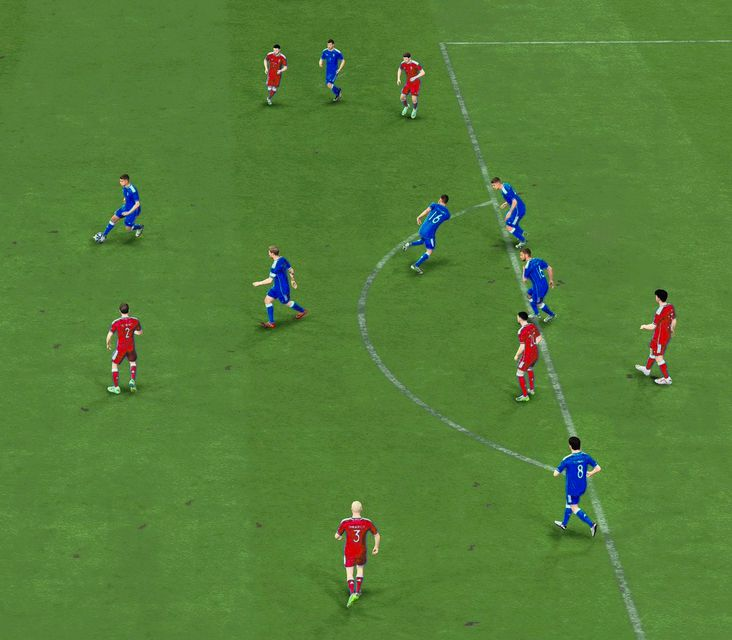
\includegraphics[width=.48\columnwidth]{vu-is-research-thesis/resources/id10_v2_b7_r6.jpg}
    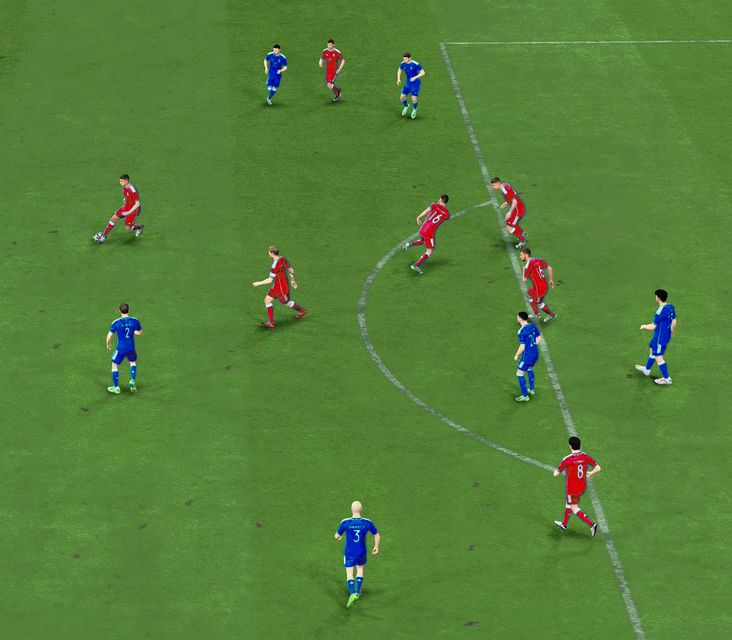
\includegraphics[width=.48\columnwidth]{vu-is-research-thesis/resources/id10_v1_b6_r7.jpg}
    \centering 
   \caption{one scene results in two stimuli where the team colours are swapped}
   \label{fitness1}
\end{figure}

\subsection{The Participant's Task}

After filling out the intake form to gather participants' relevant background information, participants are shown 60 "EAFC 24" screenshots of football players. The participants' primary task in this experiment is to make a judgment regarding which team they believe has a greater number of players in the screenshot they are shown. This task aims to gauge participants' ability to identify the majority team and quantify to what extent is the accuracy depends on jersey colour of the majority team. The mechanics of the experiment are streamlined for precision. Each screenshot is displayed for a brisk 750 milliseconds, a span allowing for instinctual, snap judgments without sufficient time to consciously count the players. Following this brief exposure, participants are prompted to indicate their choice, red or blue. Every response and response time are logged for analysis.
\section{Results}\label{s:evaluation}
\subsection{Data Processing}
To process the data for analysis, we first eliminated potentially outlying trials. On Jatos we had a total of 99 submissions, but only 49 are finished experiments. First we excluded all experiments conducted from a browser smartphone based on the operating system logged by OpenSesame and on the window with less than 750 pixels. This resulted in 4 sessions being removed, reducing the number of trials from 2940 to 2700.
Since this experiment relies on sensory memory to an extent, we eliminate trials where the response time is unreasonably long - which could happen if the subject gets distracted for whatever reason - and trials where the response time is too short - which could happen if the subject accidentally clicks the response button without having time to think about the answer. To do this, the 1st and 99th percentiles of the response times where calculated, adjusted respectively by a factor of 1.5 in order to avoid discarding valid samples. This procedure identified 4 trials below the low cutoff of 243 ms and 16 trials above the high cutoff of 7828 ms. In order to keep the data paired, in the sense that each scene is presented once with a majority blue and majority red configuration, the other version of the outlying trial was removed as well, total of 40 trials removed. Finally, we removed another session where the subject entered an age of 169. Thus the clean data set consisted of 44 sessions with 2600 trials in total.

\subsection{General overview}
In Figure \ref{stats1} we can see the distributions of age, response times, gender and football experience level of the participants as well as favourite colours. 
\begin{figure}[h!]
    \hspace{-0.5cm} % Adjust this value to move the figure to your desired position
    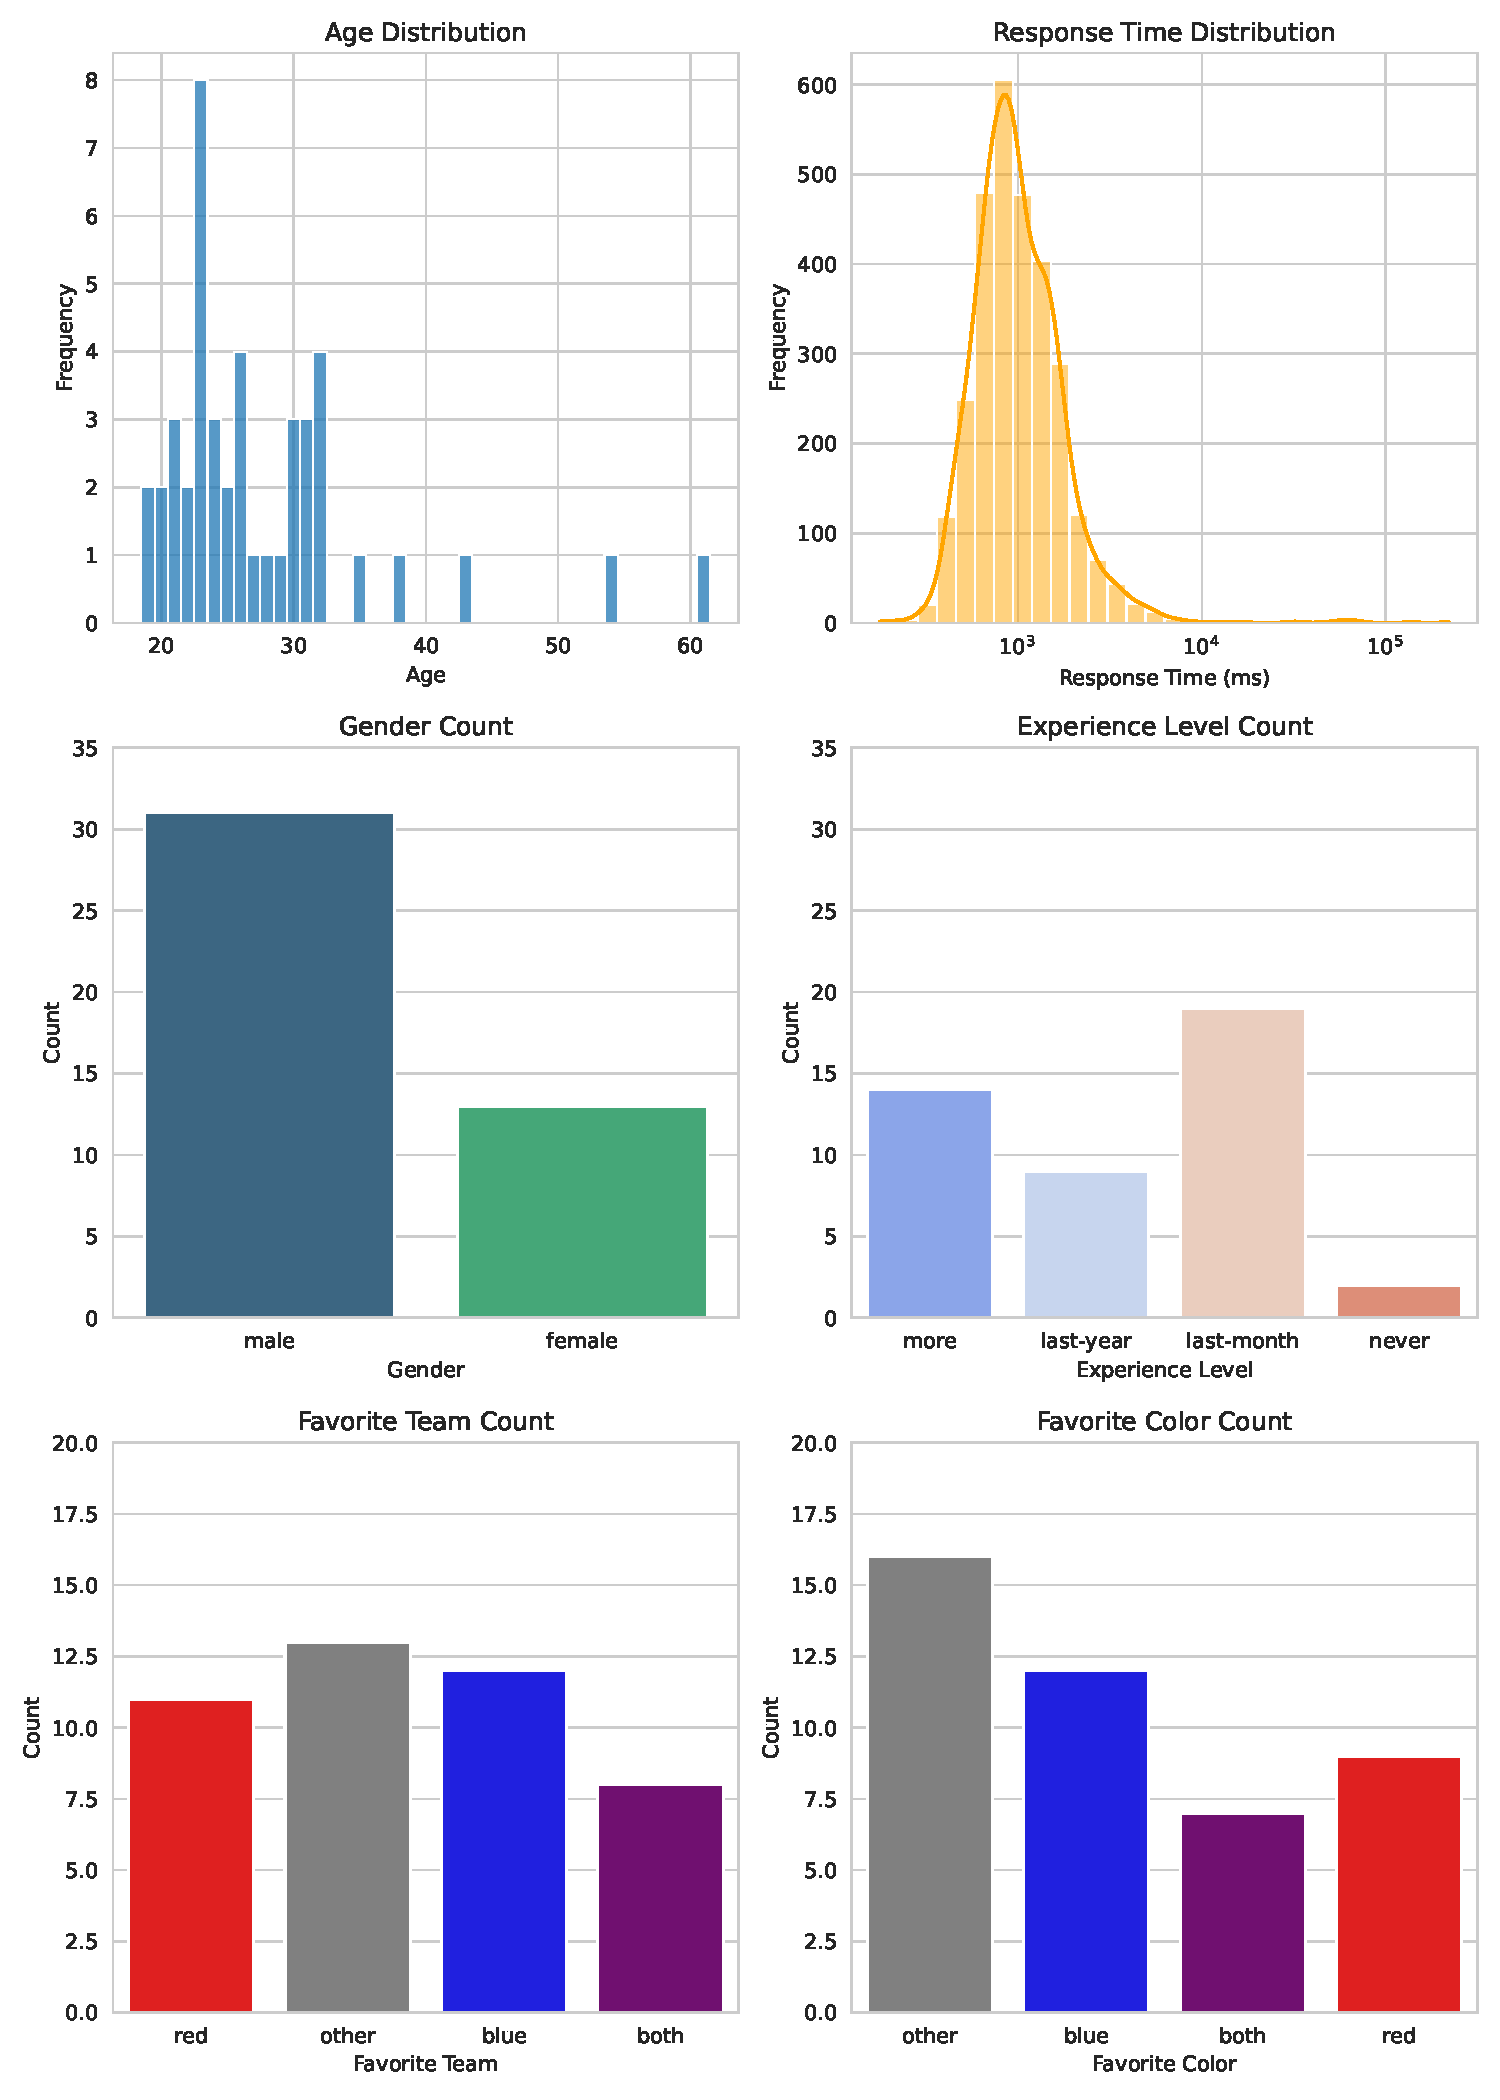
\includegraphics[width=\columnwidth]{vu-is-research-thesis/resources/demography.pdf}
   \caption{data set at a glance}
   \label{stats1}
\end{figure}
As is evident, the dataset currently skews towards younger male subjects, potentially making it more difficult to draw conclusions based on age or gender. 
% In Figure \ref{stats2}, we present an histogram of side with the most players, which serves as the correct answer (expected side) for each stimulus. We compare it them with participants' guesses, that favor the blue team more often.
% We also incorporate data on participants' favorite team colors and personal favorite colors, which we collected at the conclusion of the experiment. From the latter, it's evident that there's a minor inclination toward blue, although it's not as statistically significant as the imbalance in user responses.
\subsection{Findings}
The main research question is if the jersey colour of the majority team has an effect on accuracy. In order to investigate this question we examined the impact of various factors on accuracy. In the first row of figure \ref{stats2} it can be clearly observed that there are more trials where subjects thought that blue is the majority team compared to red, so accuracy for blue is higher. For reference, the top right plot depicts that the ground truth data is equally split between majority red and blue. 
\begin{figure}[h!]
    \hspace{-0.5cm} % Adjust this value to move the figure to your desired position
    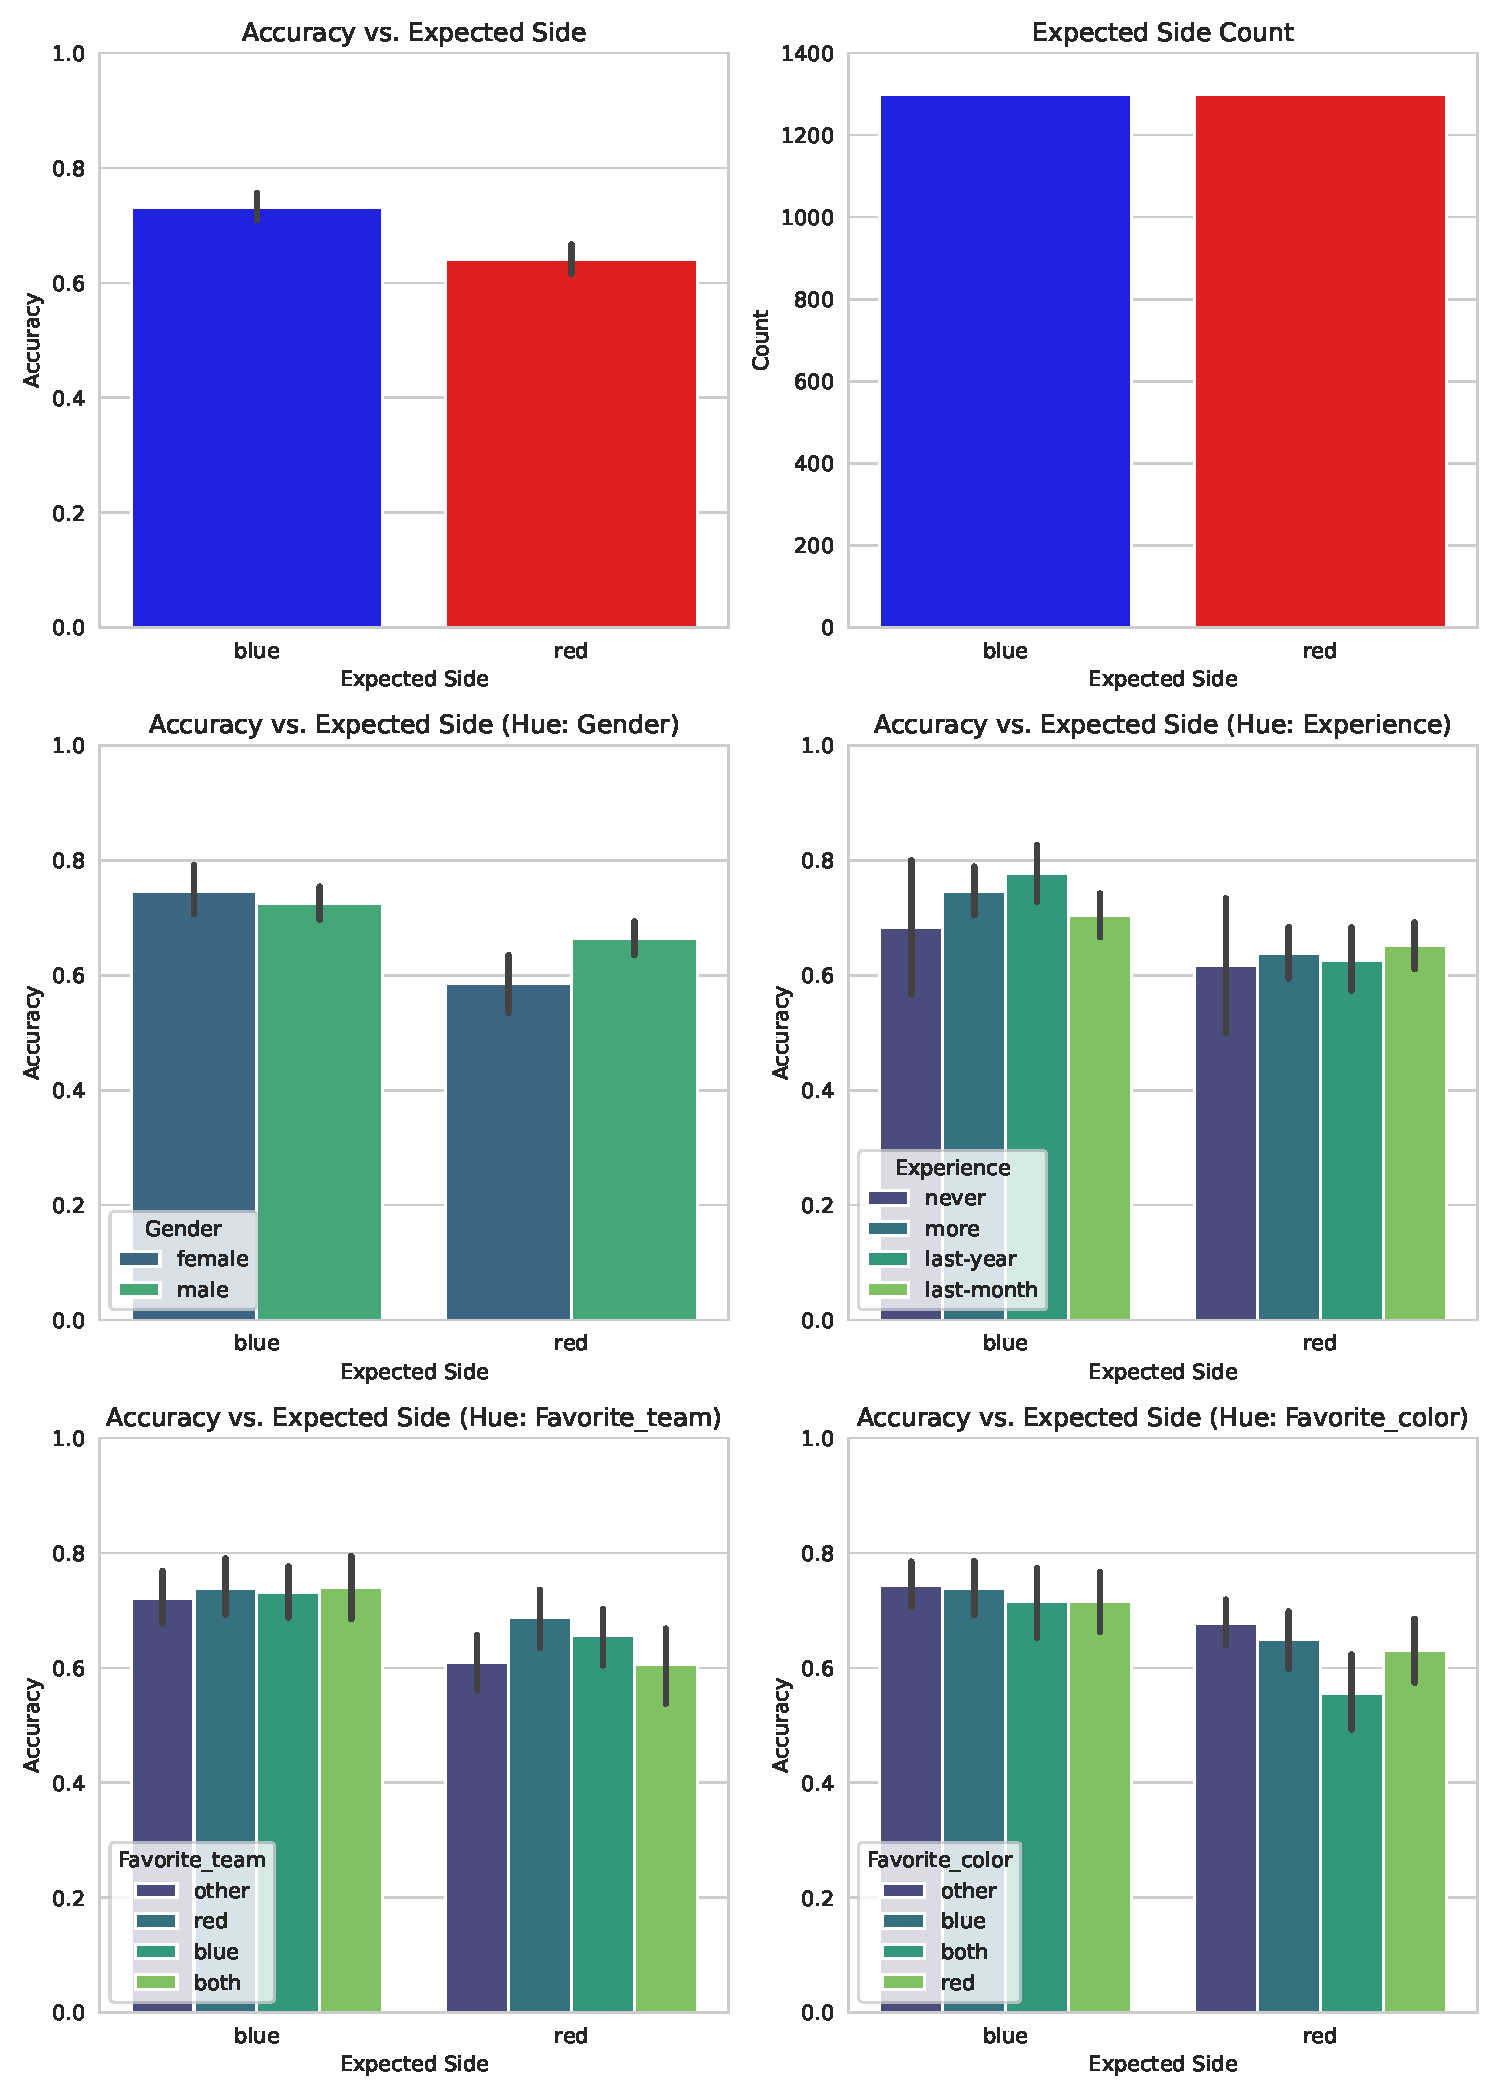
\includegraphics[width=\columnwidth]{vu-is-research-thesis/resources/accuracy_breakdown.pdf}
   \caption{accuracy breakdown}
   \label{stats2}
\end{figure}
In the next rows of figure \ref{stats2}, since the effect of expected side seems clear, the accuracy is additionally plotted by other factors. In the second row on the left the accuracy is additionally plotted by gender and on the right by experience. The by-gender breakdown seems to indicate that the effect is less pronounced for males since the difference in height for expected side blue and expected side red bars, is smaller for males. The by-experience plot indicates that the effect is least pronounced for subjects who played or watched football during the last month and the effect is much more pronounced for subject doing this one year ago or more. For the by-favourite-team and by-favourite colour plots it's not immediately clear if there is a difference given the long error-bars, the most noticeable effect perhaps being that the effect is less pronounced if the favourite team is red. The plot is just indicative of possible effects, next we will present the results of statistical tests aimed at quantifying the significance and magnitude of the effects.

\subsubsection{Models and test}

Before proceeding with more complex models, we first ran statistical tests on the contingency table of expected colour versus correctness of response. The Chi-Square test and the proportion test are applicable, and result in significant p-values (8e-7). Since the data is paired, McNemar's test is the more valid options and because the statistical power of this test is higher, it results in an even more significant p-value of 1e-8. 

Next a generalized linear model with a logistic link function is fit where the dependent variable is the $is_correct$ variable and the independent variable is only the expected (majority) side. Table \ref{table:glm_results} shows that even ignoring all other factors, the $expected\_side$ is a significant predictor of the $correct\_response$, and specifically, when the expected side is "red", the likelihood of a correct response decreases, more specifically, log odds of a correct response decrease by approximately 0.46. Given that $\operatorname{logit}\left(P_{\text {red }}\right)=\beta_0+\beta_1 \times 1=1.0024-0.4237$ the expected probability of a correct response when the majority side is red is $P_{\text {red }}=\frac{e^{\operatorname{logit}\left(P_{\text {red }}\right)}}{1+e^{\operatorname{logit}\left(P_{\text {red }}\right)}}=0.641$ and similarly $P_{\text {blue }}=0.732$. The statistical tests and the basic logistic model show beyond with great statistical certainty that subjects are biased towards blue. Next, similar to the rows of figure \ref{stats2}, several models will be presented, checking for more subtle effects.

\begin{table}[h]
    \centering
    \caption{GLM results for the effect of team color on correct response.}
    \begin{tabular}{lcccc}
        \hline
        Coeff. & Est. & Std. Error & z value & Pr(>|z|) \\
        \hline
        Intercept & 1.002 & 0.063 & 16.02 & $< 2 \times 10^{-16}$ *** \\
        expected\_side=red & -0.424 & 0.086 & -4.97 & $6.6 \times 10^{-7}$ *** \\
        \hline
    \end{tabular}
    \label{table:glm_results}
\end{table}

The basic logistic model above ignores random effects, so we ran a linear mixed-effect model (LMM) with $expected\_side$ as fixed effects and by-subject and by-scene random intercepts for the $expected\_side$ variable and we also check whether adding a random slope as well improves the model. By doing an Anova test we find that adding a random slopes doesn't significantly improve the model. Table \ref{table:glmer_results} contains the model fitted on 2600 observations where there are 44 groups for subject\_id and 30 groups for scene\_id variables.

\begin{table}[h]
    \centering
    \caption{Mixed-effects model results for the effect of team color on correct response, accounting for random effects of subject and scene.}
    \begin{tabular}{lcccc}
        \hline
        Coeff. & Est. & Std. Error & z value & Pr(>|z|) \\
        \hline
        Intercept & 1.185 & 0.177 & 6.69 & $2.2 \times 10^{-11}$ *** \\
        expected\_side=red & -0.491 & 0.091 & -5.37 & $7.9 \times 10^{-8}$ *** \\
        \hline
    \end{tabular}
    \label{table:glmer_results}
\end{table}

The variance for the random effect of subject (\textit{subject\_id}) is 0.252, indicating a moderate degree of variability in correct responses across subjects. The variance for the random effect of scene (\textit{scene\_id}) is 0.621, indicating a higher degree of variability in correct responses across different scenes. We note that considering the random effects the significance of the difference between the log odds of correct responses for red and blue majority trials becomes more significant by an order of magnitude.

Table \ref{table:glmer_results_interaction} summarises the model which considers genders as an additional fixed effect, in interaction with expected side. This model quantifies the difference depicted in figure \ref{stats2} middle left. This model, shows that while gender by itself is not a good predictor of accuracy, its effect becomes significant as an interaction with the expected side. In other words, the effect of expected side on accuracy is not the same for males and females. More specifically, the expected log odds of a correct answer for a female subject is 1.253 for a majority blue sitmulus but odds decrease significantly by 0.838 when the expected side is red to 0.415. The expected log odds for a male when majority blue is 0.098 lower than a female, but this difference is not significant, but when the majority is red, the expected log odds of correct response rise to 1.253 - 0.098 + 0.410 = 1.655.
\begin{table}[h]
    \centering
    \caption{GLMM results for the effect of team color and gender on correct response, with random effects of subject and scene.}
    \begin{tabular}{lcccc}
        \hline
        Coeff. & Est. & Std. Error & z value & Pr(>|z|) \\
        \hline
        Intercept & 1.253 & 0.236 & 5.31 & $1.1 \times 10^{-7}$ *** \\
        e\_s=red & -0.838 & 0.166 & -5.03 & $4.8 \times 10^{-7}$ *** \\
        gndr=male & -0.098 & 0.221 & -0.44 & 0.657 \\
        e\_s=red:gndr=male & 0.410 & 0.199 & 2.51 & 0.012 * \\
        \hline
    \end{tabular}
    \label{table:glmer_results_interaction}
\end{table}
Finally, we check favourite colour, favourite team and experience as covariates in interaction with expected side but do not find statistically significant effects. Some interesting qualitatitive observations can be made based on these figures. While the response time distributions are basically identical for blue/red expected sides which is interesting because it indicates that the duration of the cognitive mechanisms which leads to the estimation bias is not itself affected by the majority colour. A subtle difference in the distributions can be observed for correct and incorrect responses, where incorrect responses tend to have more shorter response times and more longer response times. Perhaps most intriguingly, the RT distribution is significantly different between males and females, where female subjects not only tend to respond slower on average, but the response time is also bimodal. 

\subsubsection{Response times}
In addition to the accuracy, a secondary investigation can be performed on the response times. In particular figure \ref{stats3} depicts the response times for correct/incorrect responses, male/female subjects and blue/red expected sides.
\begin{figure}[h!]
    \hspace{-0.5cm} % Adjust this value to move the figure to your desired position
    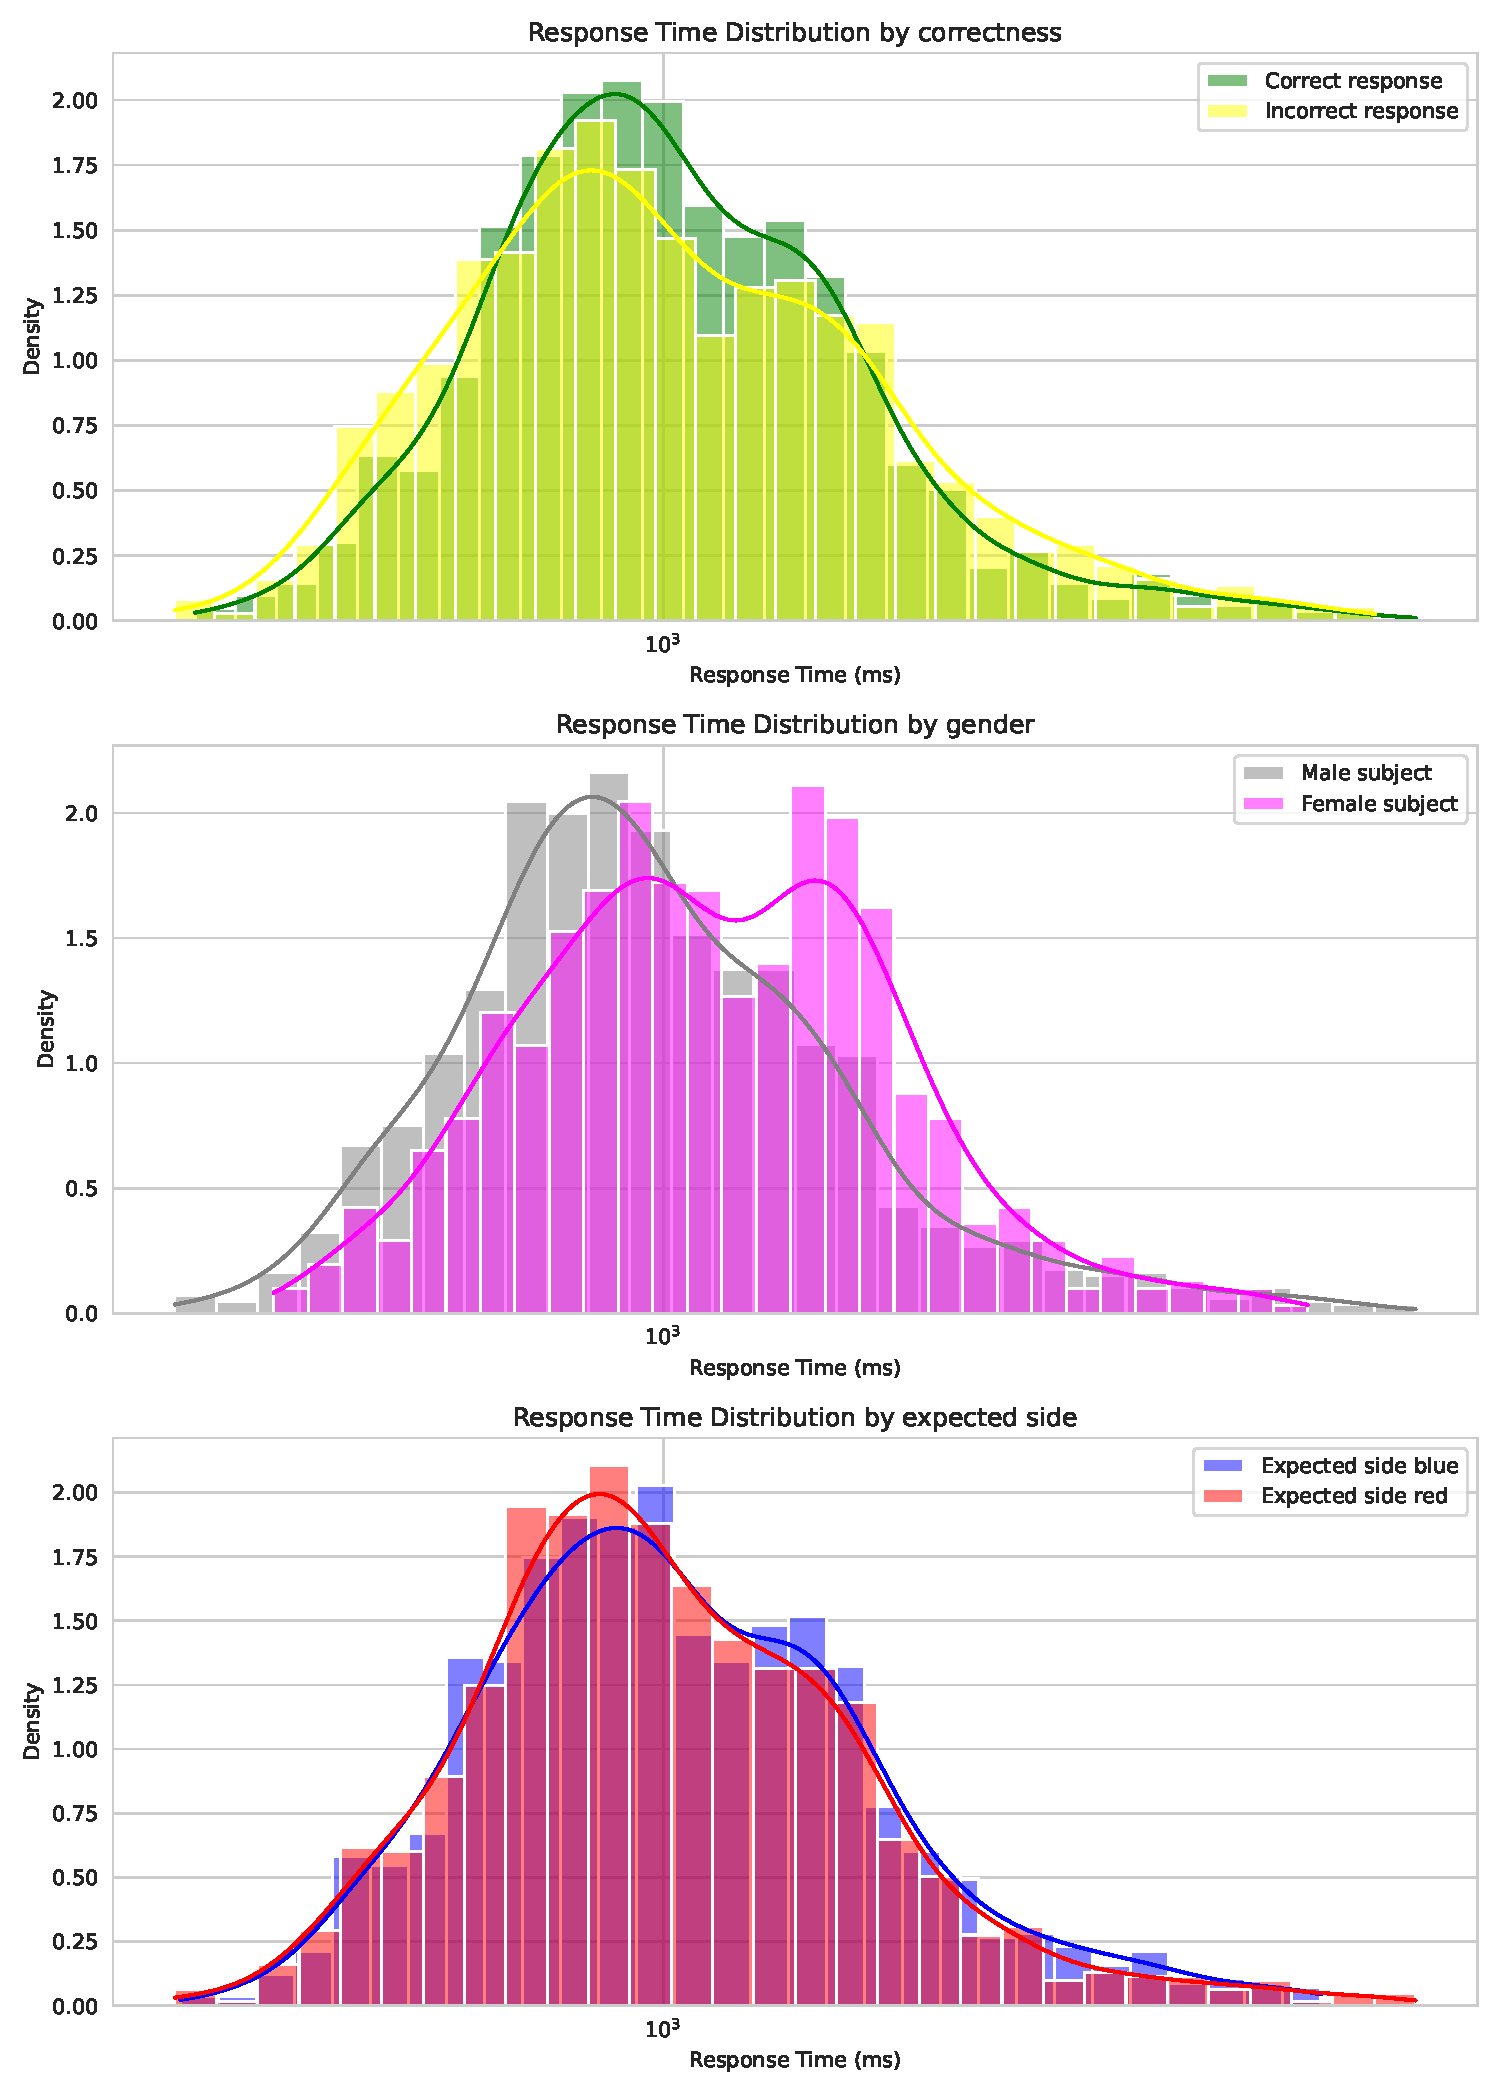
\includegraphics[width=\columnwidth]{vu-is-research-thesis/resources/response_times.pdf}
   \caption{response time distributions}
   \label{stats3}
\end{figure}
While the response time distributions reveal interesting avenues of further investigation, given the current data, it is not immediately clear how the response time data can be interpreted to explain the color salience research question.
\section{DISCUSSION}\label{s:discussion}

The fascinating conclusion from this study is that the experimental results show the opposite effect to the initial hypothesis. The initial hypothesis states that the psychological salience of red as a color related to danger and aggressiveness would prompt subjects to overestimate the presence of red players. The experimental results show that subjects overestimated the presence of blue players. We provide a few speculative explanations for this behavior below.

\subsection{Results Explanations}

One possible explanation is a failure of the assumption that higher salience means higher numerical estimates. It could be that red still has a higher salience, which leads to more accurate counts of red players, and that the lower salience of blue actually leads subjects to overestimate the number of blue players due to the inability to accurately count them. This would indicate a bias towards overestimating objects that receive low cognitive attention, a plausible, conservative, survival mechanism. This theory could be tested with a similar experiment where the subjects are tasked to estimate the counts of salient and non-salient objects, perhaps by manipulating the contrast on a fixed background. If the counts of non-salient objects are consistently overestimated it would explain the result in this study, while upholding the assumption that red is the more salient color. One confounding effect to consider in this proposed experiment is the natural bias of each subject, some subjects might overestimate when faced with uncertainty, while others might underestimate. This effect could be studied by providing an intuition-based numerical guessing task for each subject and tracking the effect of uncertainty in numerical guessing.

Another possible explanation is that blue might have a higher natural salience of its own. This salience can be biological, related to ocular receptors and wavelengths, or psychological. Red's psychological salience is well-researched and is often exploited in modern visual signals. Blue also has a likely psychological salience of its own kind, it is a color rarely found in land organisms, but often associated with water and the sky, two features that humans might intuitively search for. Blue's salience is also used in road signs, particularly in the European Union, which is a testament to its ability to draw attention. Perhaps this alternative psychological salience counteracts the salience of red and leads to a bias towards blue estimates. This theory could be tested by performing a study with more diverse colors, always including red and blue, and investigating where blue and red stand in a ranking of salience, if both blue and red place similarly in salience, perhaps this study is affected by two highly salient colors.

A final explanation to consider is some confounding effects due to the experiment design. One possible point of conflict is the labeling of buttons for "red" and "blue" with the color of the respective option. This is a visual guide to avoid errors in the button clicking. Perhaps red's association with danger and aggressiveness leads subjects to be more hesitant towards choosing the red option, creating a bias towards the more agreeable color, blue. This confounding effect can be studied with an additional experiment testing bias between red and blue labeled buttons, or by repeating this study without coloring the buttons.

Another interesting finding is that the effect size is stronger for females. This could point to a psychological effect imbued by societal norms or could be a factor of the different sample sizes of males vs females. This finding should also be studied further, with studies that focus on the differences in biases and attention to blue and red, based on sex and gender. Such a study could determine whether there is a biological or a socio-psychological effect on color-based attention. The results also show that the effect is larger for subjects who have never played football. Given football in Europe has traditionally been more popular among males, this might explain why the effect is larger in females. This study could be repeated with a focus on tracking familiarity with football as an independent variable, to check if it is correlated to gender and the effect on player detection.


\subsection{Applicability to the real world}
The findings in this paper could explain the red-advantage effect in football \cite{english}. The amount of players wearing red is often underestimated, this adds a component of stealth that can be exploited by players. In fact, the original assumption that red's psychological salience leads to the overestimation of player counts, makes the red-advantage effect harder to justify. Overestimating opposing red players could lead to more conservative play and stop potentially good plays, but underestimating red players is likely to lead to mistakes and lost balls which are often more detrimental. A further study should be done to verify which of these effects is more beneficial to team performance, being numerically overestimated or numerically underestimated. If such an effect is significant, clothing colors should be increasingly taken into account to improve competitiveness and fairness.

Another interesting use of this finding is in signaling techniques, where we can exploit the presence of blue being overestimated.  Any situation that uses red to signal several dangers or measurements could be switched to blue if a less accurate and more conservative perception is desirable. For instance, red lights are often used in aviation to signal obstacles, using blue lights might lead to a more conservative estimation of the danger of an area, leading to safer flying. Another example is the bars with red and white stripes that are often used as barriers for cars. Perhaps using blue and white stripes will lead to the bar being perceived as longer, avoiding collisions.


% \input{sections/threats}
% \input{sections/related}
\section{Conclusion}\label{s:conclusion}

In this research we have explored the influence of colour on the saliency of football players. Motivated by the real-life relevance in football, we have focused on one specific interpretation of saliency, namely relative majority in a scene. We have formulated a specific research questions, we asked if subjects' ability to identify the majority team depends on the jersey colour of the majority team. We picked red and blue because they are commonly used in football and commonly studied in related cognitive psychology research. Our experimental results clearly show a noticeable and significant effect of jersey colour on subject accuracy. Our subject reported blue as the majority team significantly more so than they did red. While the cognitive mechanisms explaining our results warrant further investigation, the experimental results are difficult to refute.

\bibliographystyle{ACM-Reference-Format}
\clearpage
\bibliography{references}

\end{document}


%%% Local Variables:
%%% mode: latex
%%% TeX-master: t
%%% End:
